% !TEX root = ../main.tex
\section{Experiments} \label{sec:experiments}

In this section,
we carry out a simulation study to compare
the Bayesian coverage of credible intervals
from Gaussian approximations to two different targets.
The Gaussian distributions were parametrized by mean
and log standard deviation,
which is more numerically stable.
In each simulation study,
we minimized both the reverse and the forward KL divergence
using 10,000 iterations of stochastic gradient descent
with learning rate $\propto 1/\sqrt{t}$;
the proportionality constant was fine-tuned for every experiment.
The code to reproduce our experiments is available at .


\subsection{Cauchy} \label{subsec:cauchy}

First we consider approximating a Cauchy distribution
$\pi(x)=(\pi(1+x^2))^{-1}$.
This example was chosen because it gives us access to exact
credible intervals and also because of its heavy tails,
which should encourage the reverse KL-optimal
approximation to severly underestimate the variance
and viceversa with the forward KL-optimal approximation.
This is seen in \cref{fig:cauchy_lp},
where the tails of $q_\mathrm{fwd}$ are a better
approximation to those of $\pi$.
\cref{fig:cauchy_lims,fig:cauchy_coverage}
show the limits and resulting coverage of each approximation.
As expected, the $q_\mathrm{fwd}$ tends to have better coverage,
especially for large credibility values.
Specifically, for $\alpha=0.05$
the coverage is nearly exact.
On the other hand, $q_\mathrm{rev}$ produces
intervals with consistently low coverage.

\begin{figure}[ht]
    \begin{subfigure}{\linewidth}
    \centering
    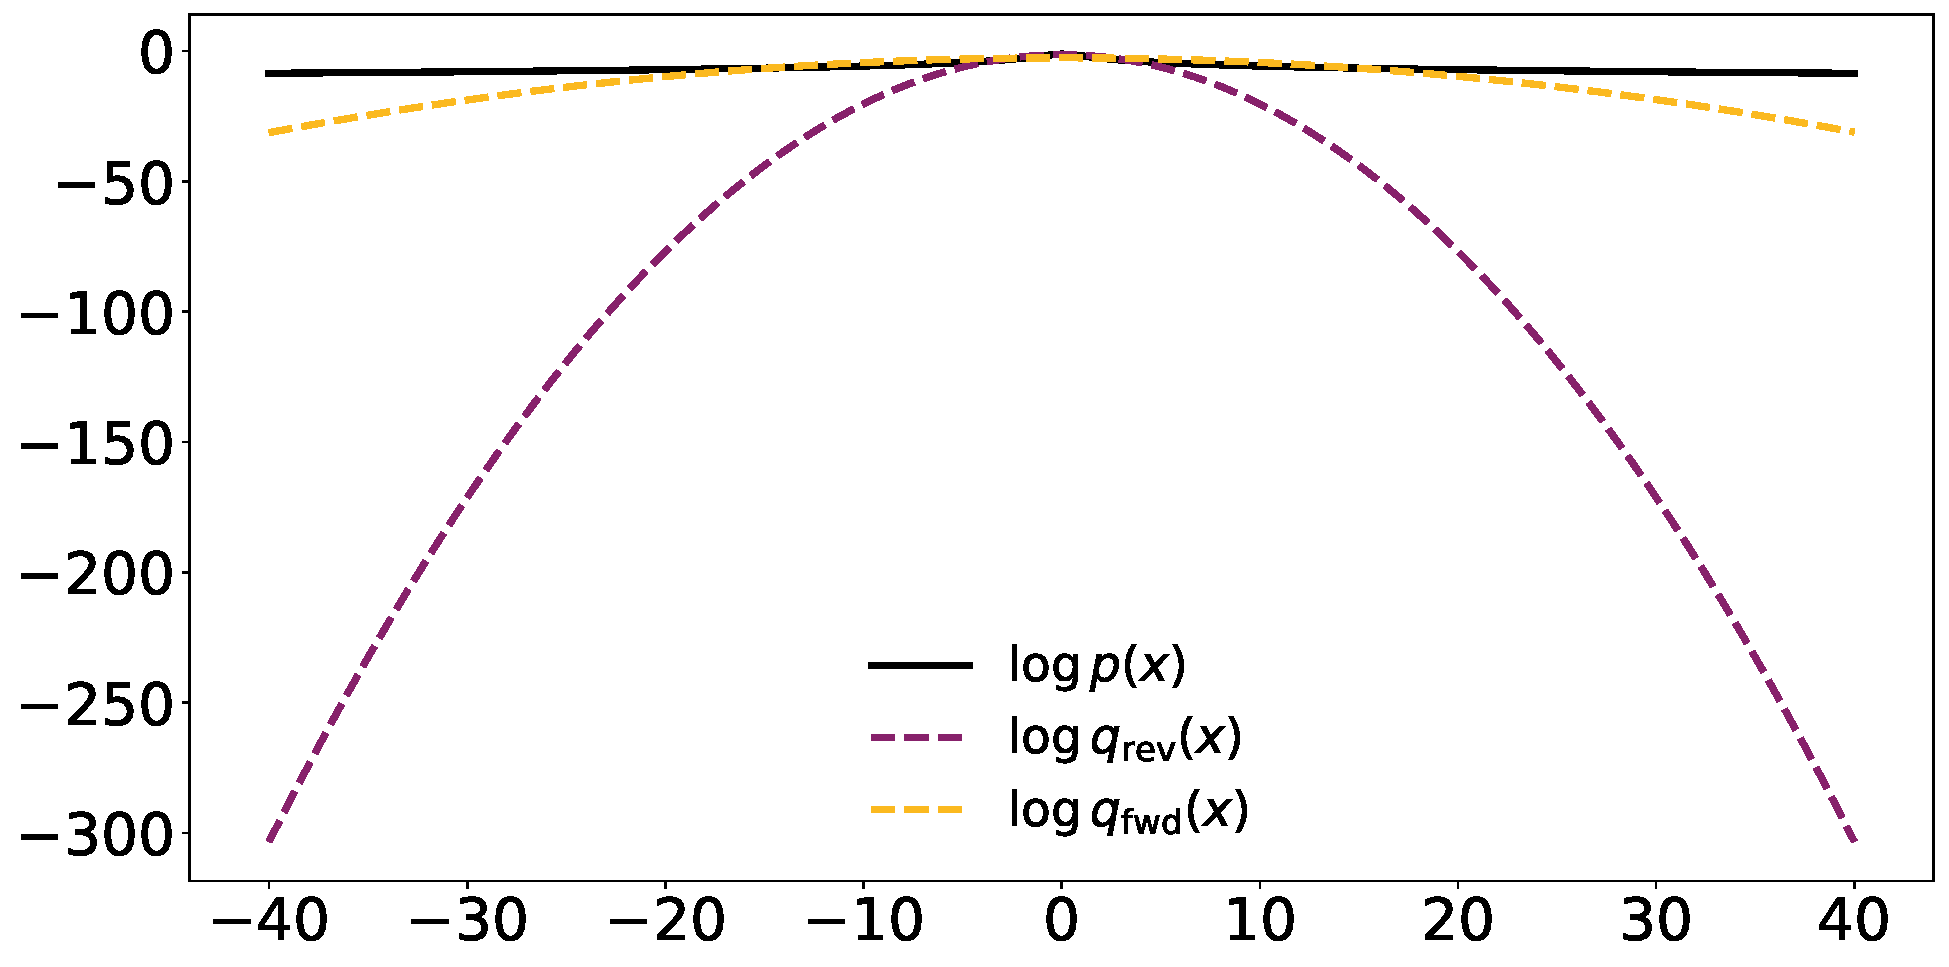
\includegraphics[width=0.8\linewidth]{fig/cauchy_logq.pdf}
    \caption{Log density}
    \label{fig:cauchy_lp}
    \end{subfigure}\\[1ex]
    \begin{subfigure}{\linewidth}
    \centering
    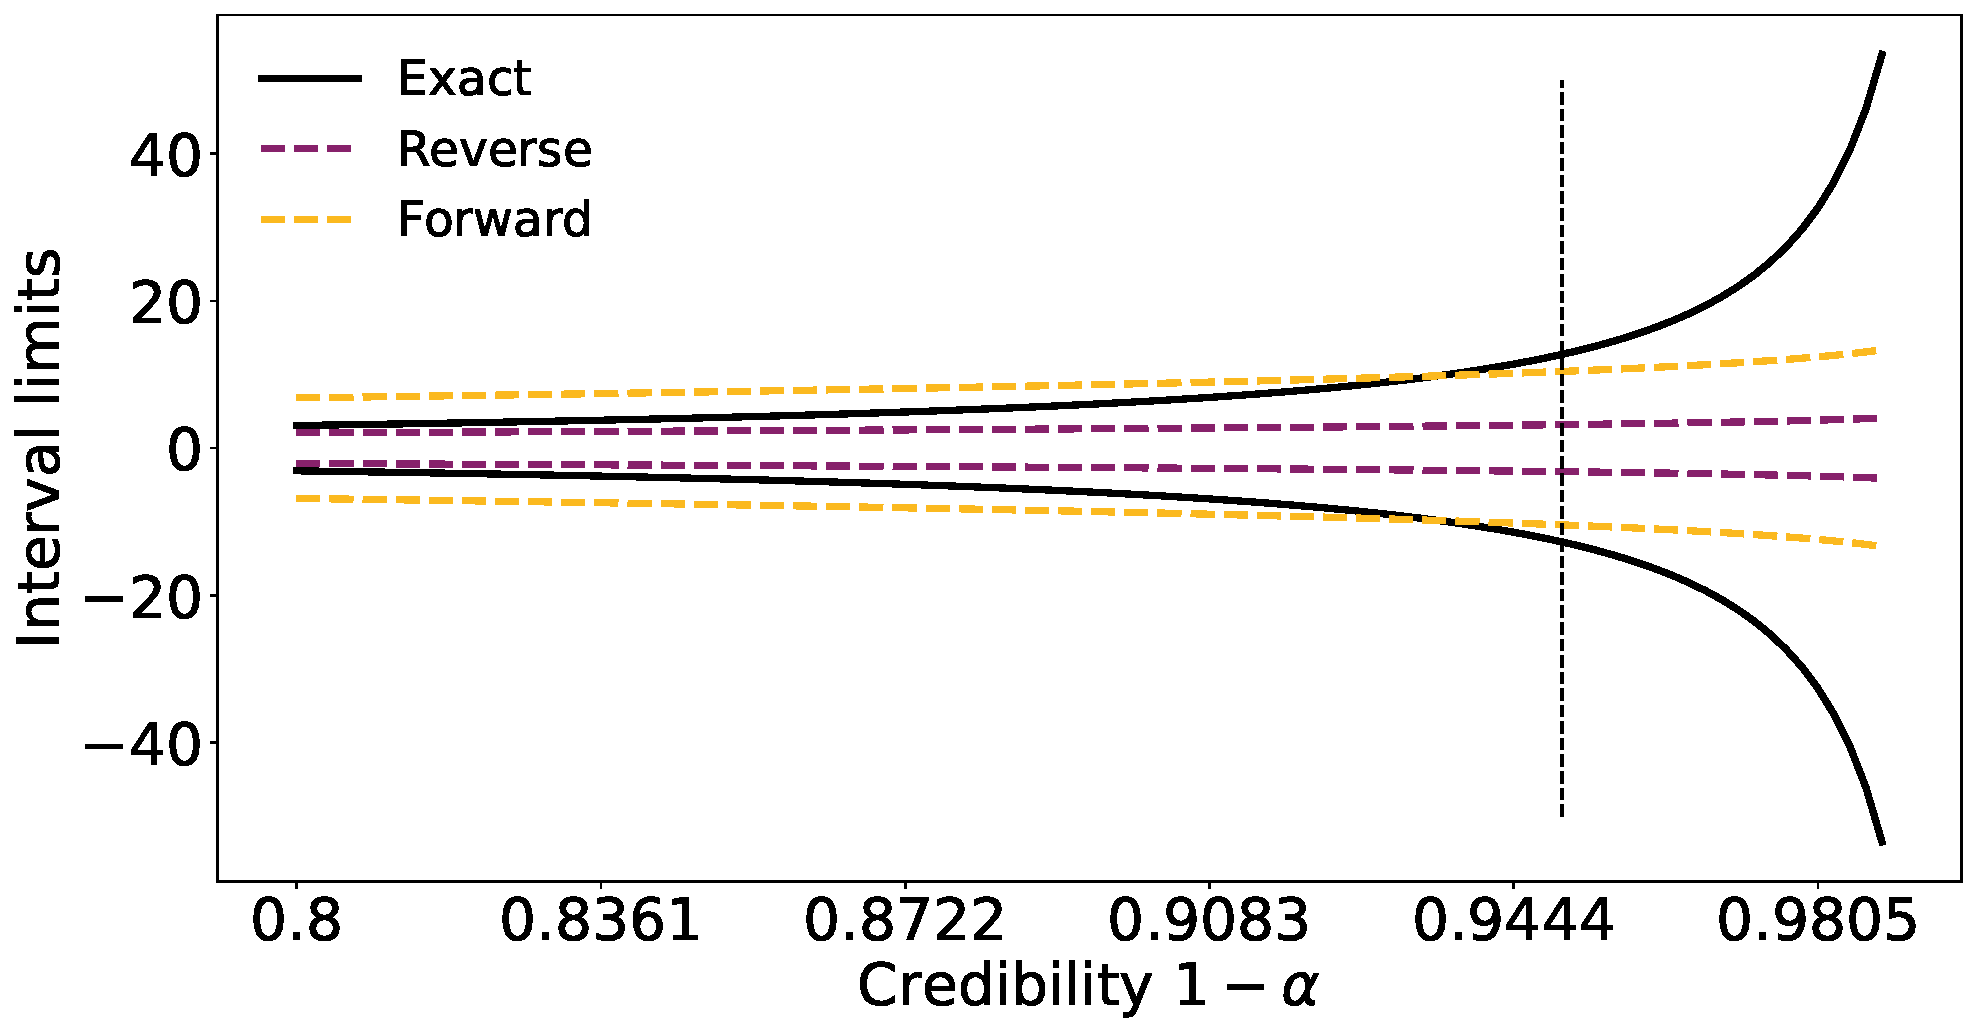
\includegraphics[width=0.8\linewidth]{fig/cauchy_cilims.pdf}
    \caption{CI limits}
    \label{fig:cauchy_lims}
    \end{subfigure}\\[1ex]
    \begin{subfigure}{\linewidth}
    \centering
    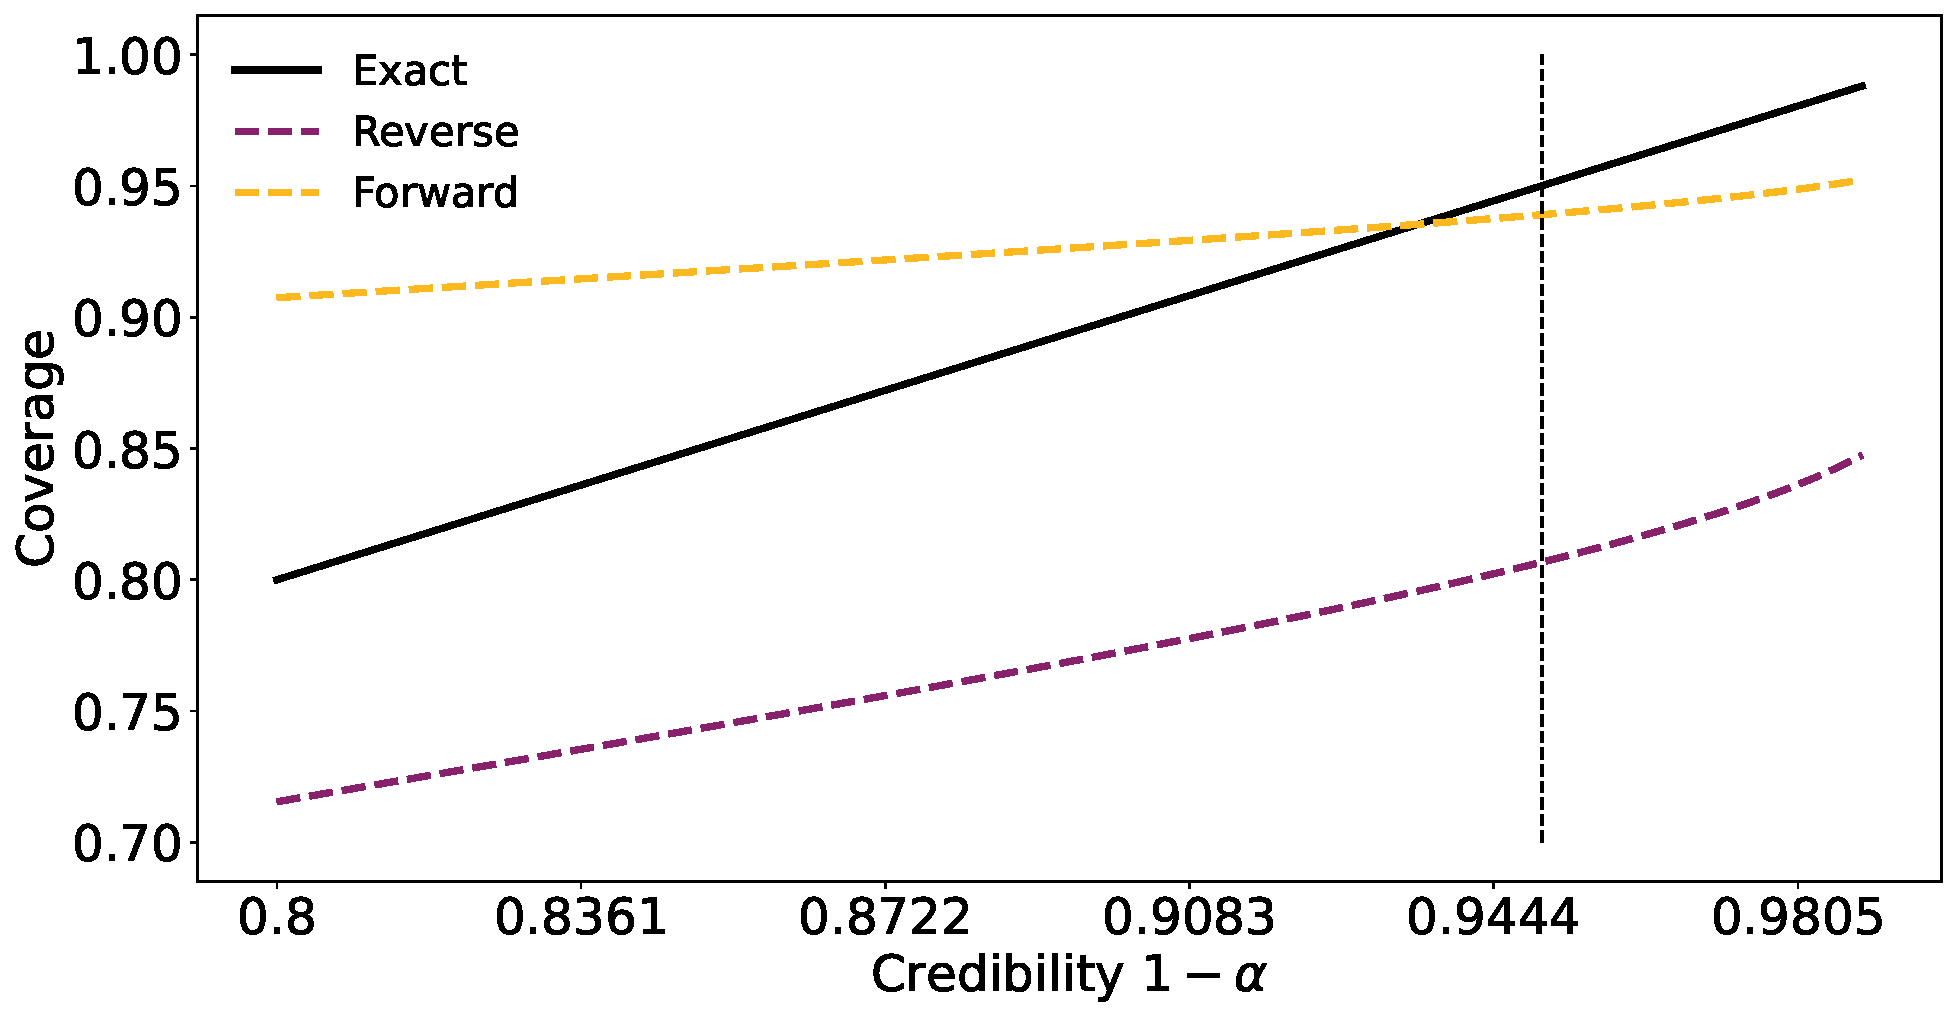
\includegraphics[width=0.8\linewidth]{fig/cauchy_cicoverage.pdf}
    \caption{CI coverage}
    \label{fig:cauchy_coverage}
    \end{subfigure}
    \caption{Results on the Cauchy distribution.}
    \label{fig:cauchy}
\end{figure}



\subsection{Logistic regression} \label{subsec:logreg}


Now we consider a logistic regression example where
we observe $N=100$ observations from the model
\[
  Y_n\sim\distBern(p_n),\quad
  p_n=\frac{1}{1+\exp\{-\beta_0-\beta_1 x_1\}},\quad
  x_n\sim\distNorm(-1,1.5^2).
\]
We set $\beta=(2,3)$ and assumed that $\beta_0=2$ is known,
so we only approximate the posterior distribution of $\beta_1$.
We estimated the normalizing constant $Z$ using
a simple numerical approximation to the integral.
The posterior distribution is unimodal and symmetri,
and thus should be well-approximated by a Gaussian,
but it has a slightly heavy right tail.
We also ran Hamiltonian Monte Carlo for 10,000 iterations
using Stan to assess the fidelity of
$q_\mathrm{rev}$ and $q_\mathrm{fwd}$.
\cref{fig:logreg_p} shows the resulting densities.
The forward KL-optimal approximation seems to be the better fit,
and it also better captures the right-tail of the target
as seen in \cref{fig:logreg_lp}
(although neither it nor $q_\mathrm{bwd}$ do an amazing job).
In terms of the interval limits,
the light left tail is well approximated by both VI densities
and by the MCMC samples,
but the heavier right tail results in
credible intervals with smaller lower limits,
as seen in \cref{fig:logreg_lims}.
All methodologies result in intervals with smaller-than-nominal coverage,
although $q_\mathrm{fwd}$ does have the coverage closest to nominal
for credibility values larger than 0.05; see \cref{fig:logreg_coverage}.
This is potentially due to the slight over correction
in the lower limit of the interval in \cref{fig:logreg_lims}.


\begin{figure}[ht]
    \begin{subfigure}{0.475\linewidth}
    \centering
    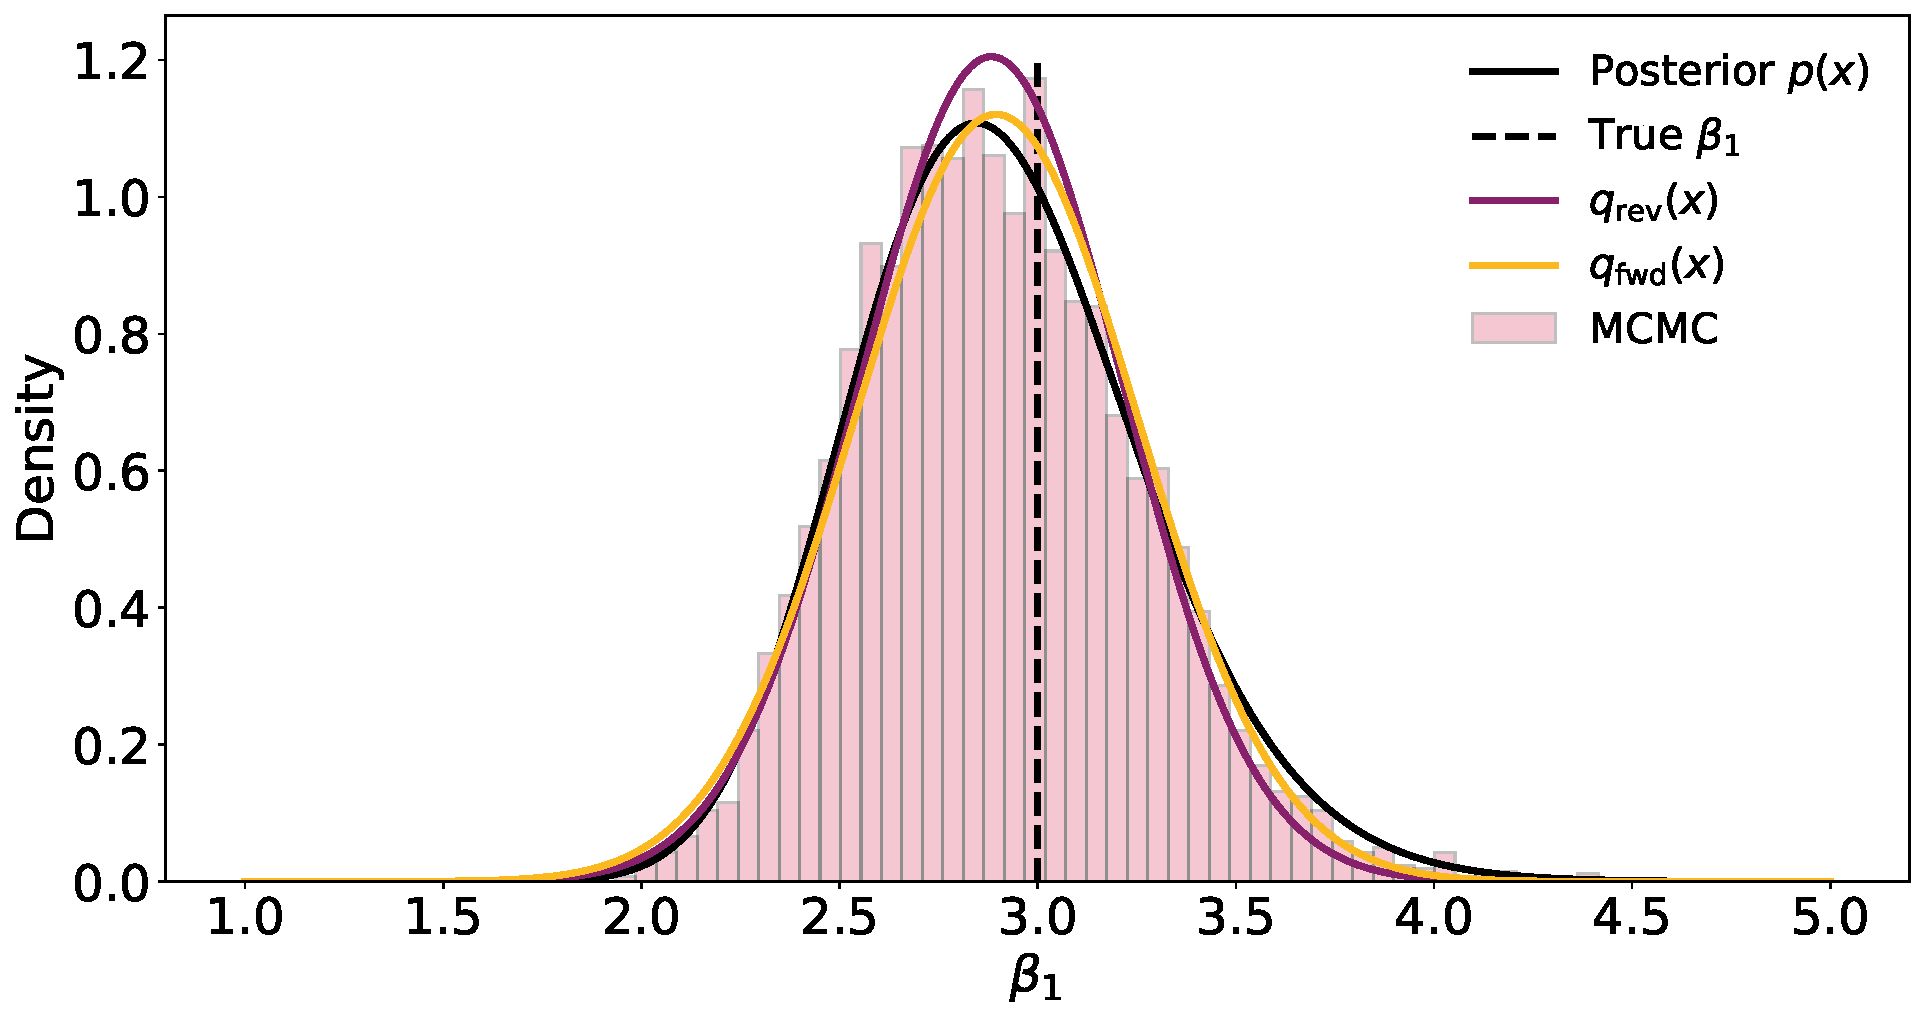
\includegraphics[width=\linewidth]{fig/logreg_q.pdf}
    \caption{Density}
    \label{fig:logreg_p}
    \end{subfigure}%
    \begin{subfigure}{0.475\linewidth}
        \centering
        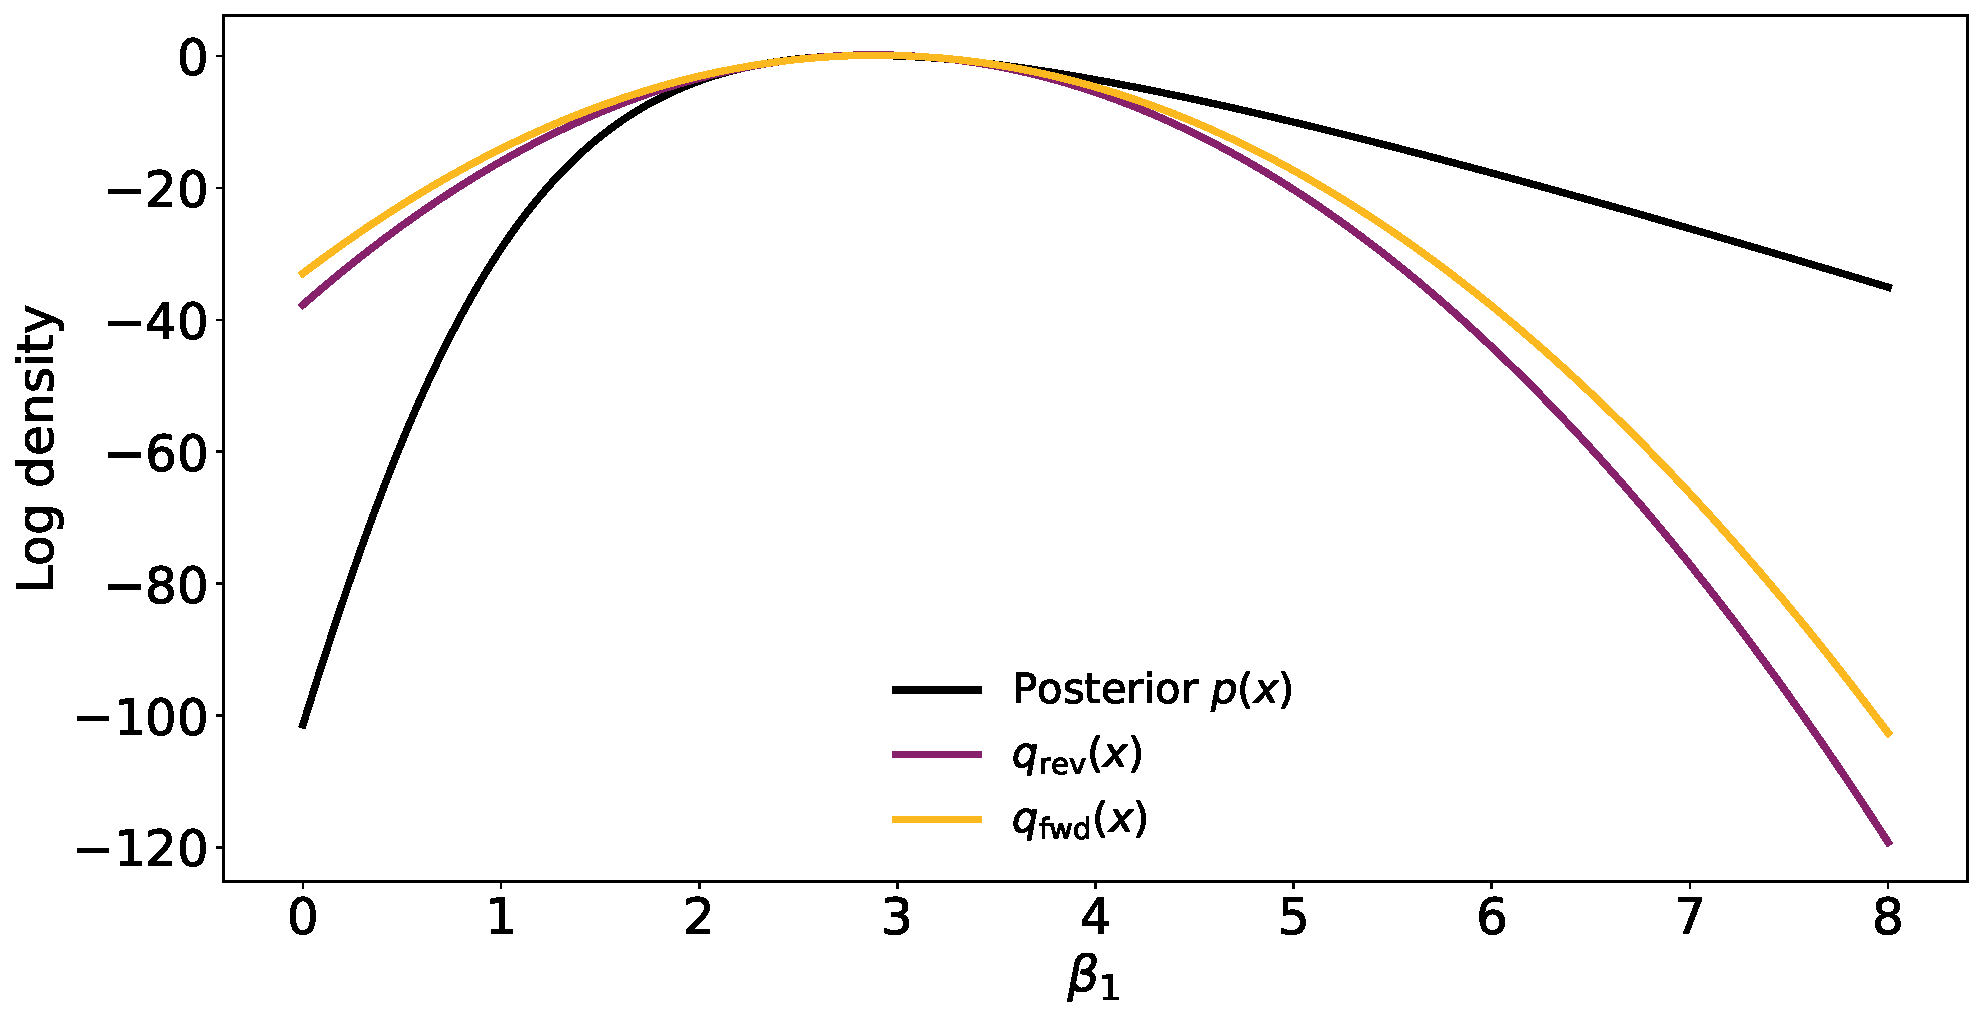
\includegraphics[width=\linewidth]{fig/logreg_logq.pdf}
        \caption{Log density}
        \label{fig:logreg_lp}
        \end{subfigure}\\[1ex]
    \begin{subfigure}{\linewidth}
    \centering
    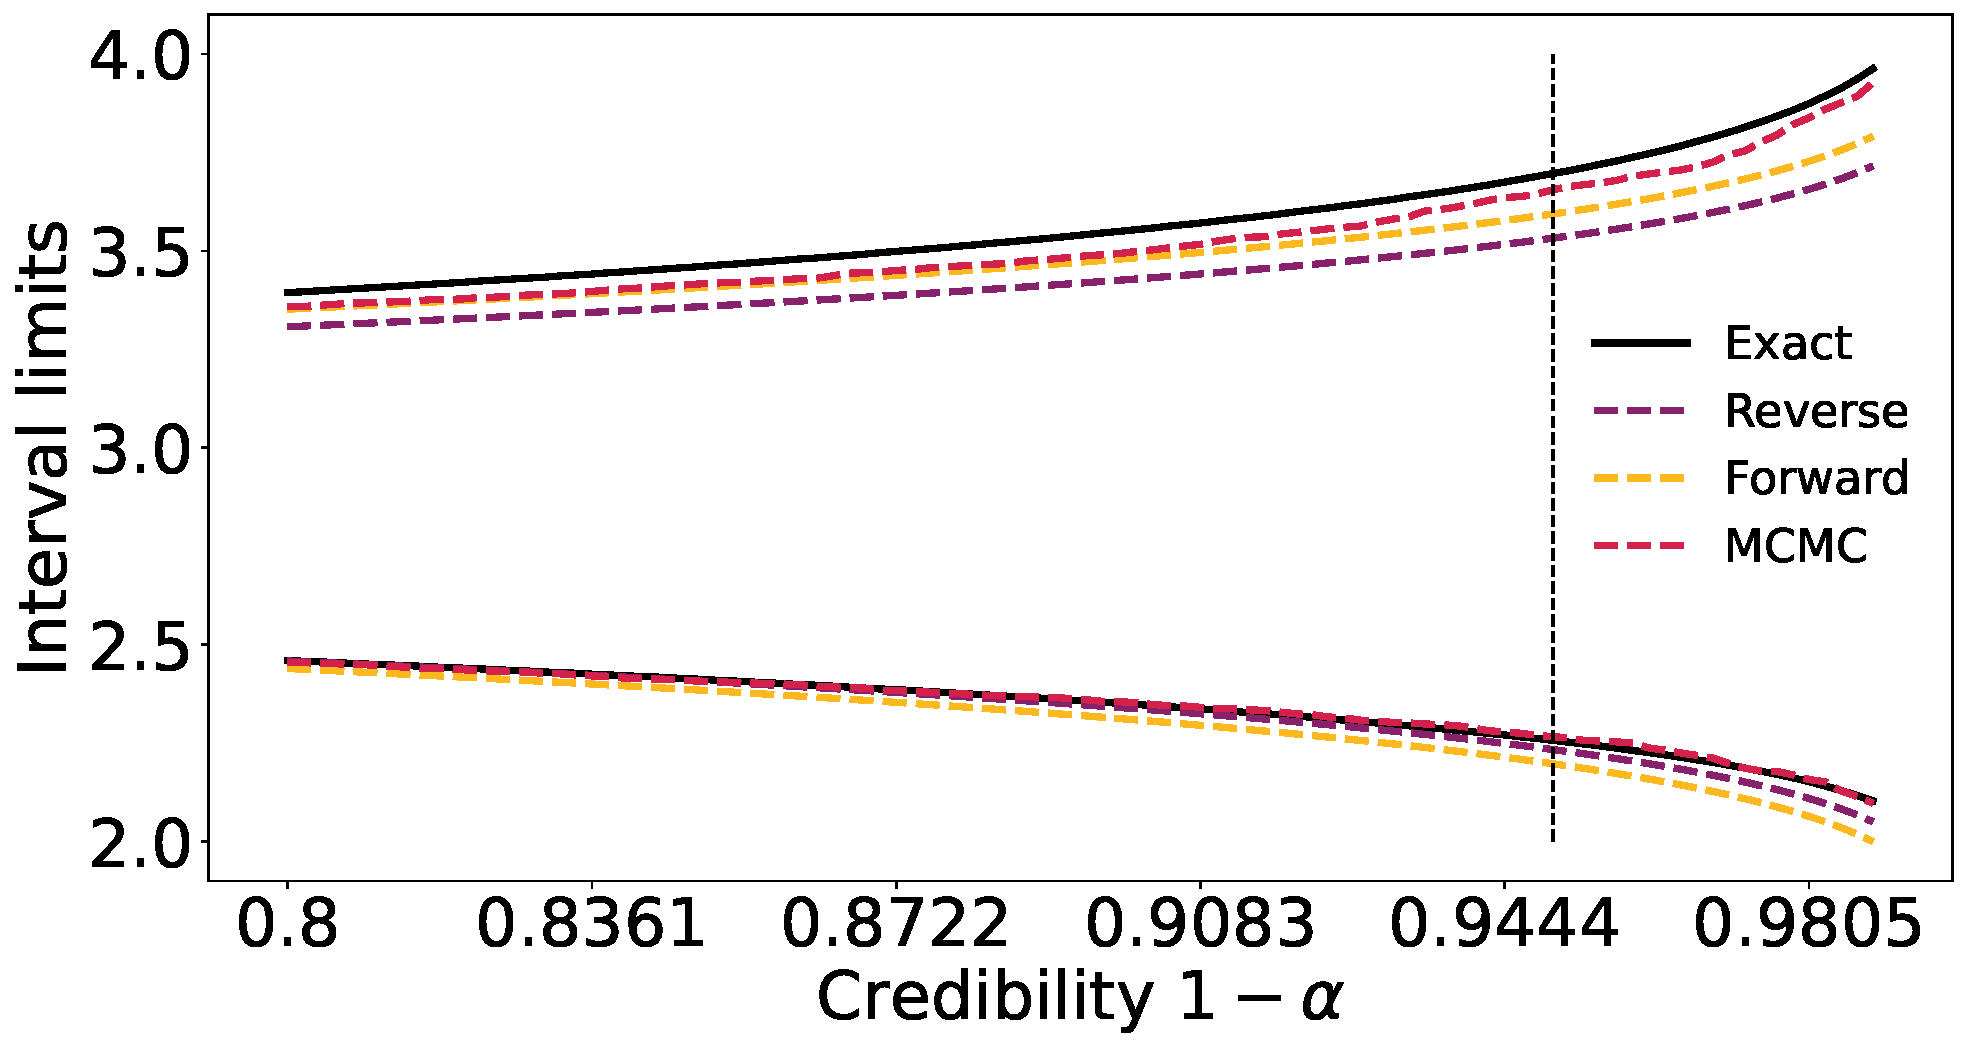
\includegraphics[width=0.8\linewidth]{fig/logreg_cilims.pdf}
    \caption{CI limits}
    \label{fig:logreg_lims}
    \end{subfigure}\\[1ex]
    \begin{subfigure}{\linewidth}
    \centering
    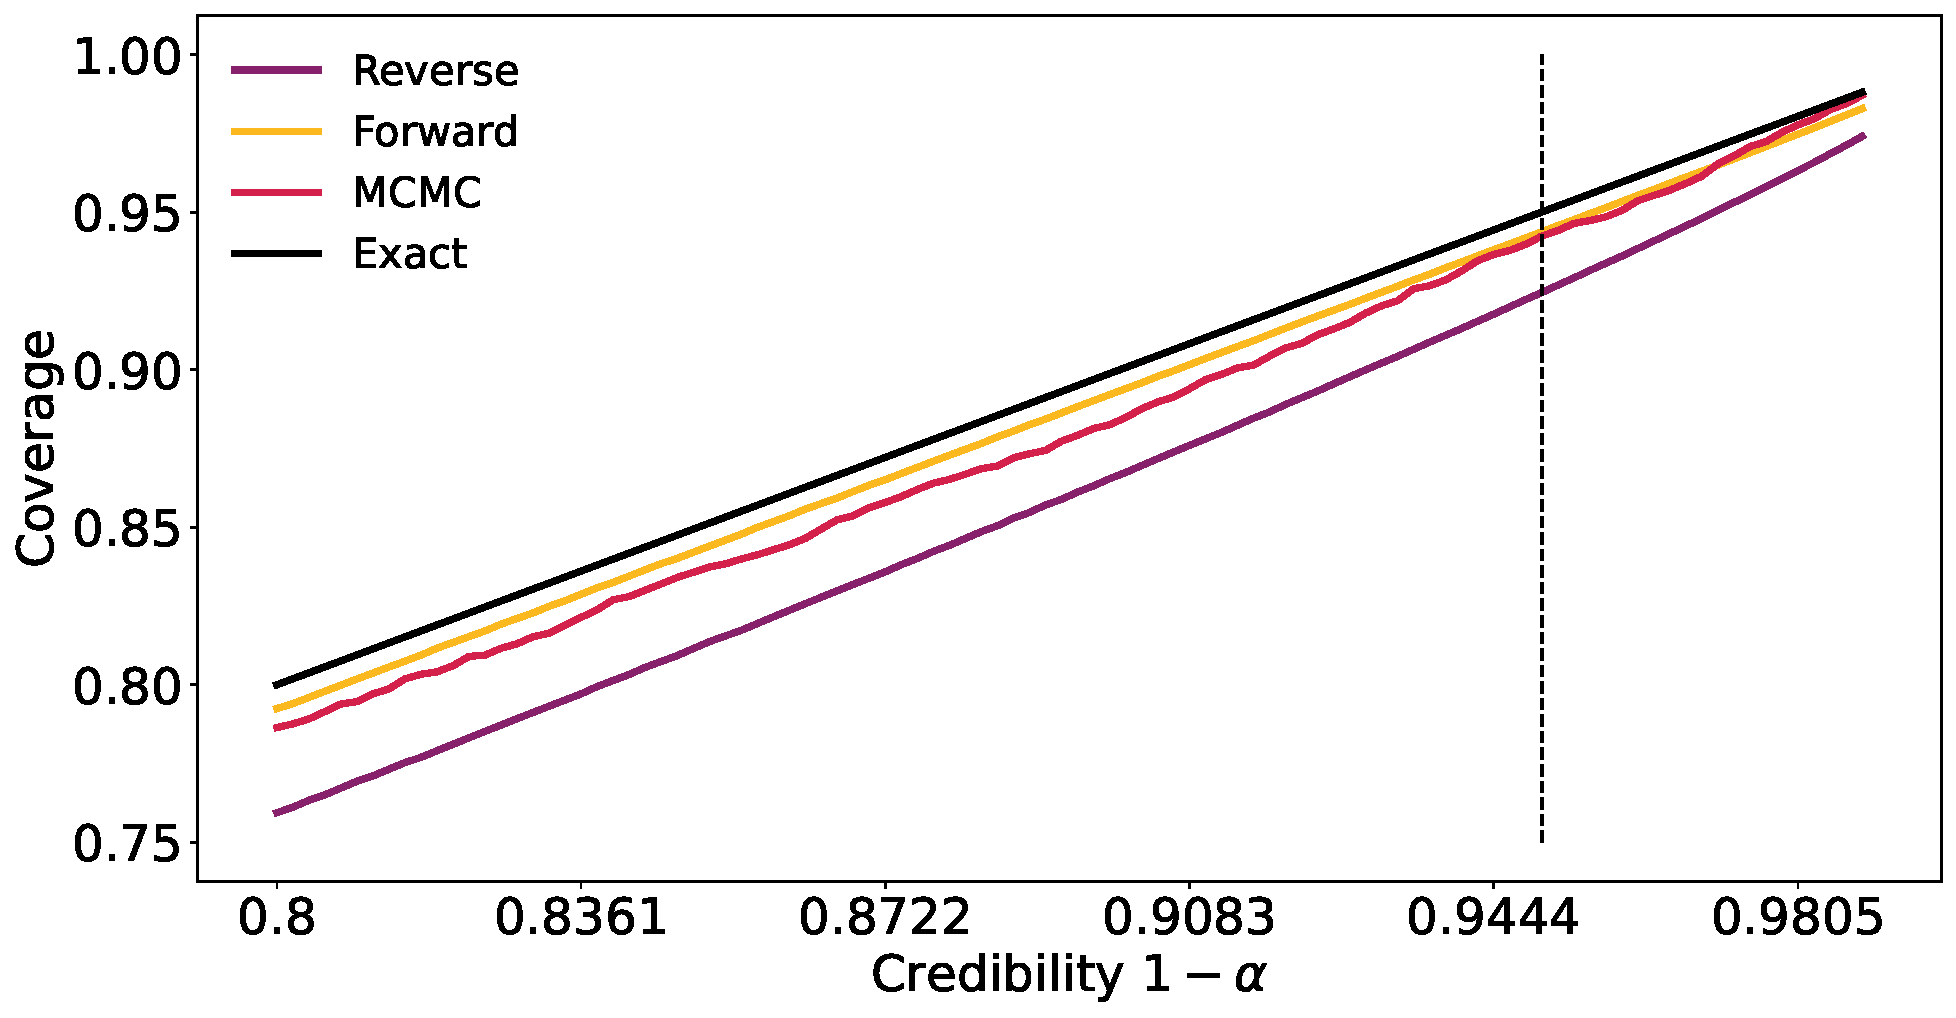
\includegraphics[width=0.8\linewidth]{fig/logreg_cicoverage.pdf}
    \caption{CI coverage}
    \label{fig:logreg_coverage}
    \end{subfigure}
    \caption{Results on the logistic regression example.}
    \label{fig:logreg}
\end{figure}
